\documentclass[1p]{elsarticle_modified}
%\bibliographystyle{elsarticle-num}

%\usepackage[colorlinks]{hyperref}
%\usepackage{abbrmath_seonhwa} %\Abb, \Ascr, \Acal ,\Abf, \Afrak
\usepackage{amsfonts}
\usepackage{amssymb}
\usepackage{amsmath}
\usepackage{amsthm}
\usepackage{scalefnt}
\usepackage{amsbsy}
\usepackage{kotex}
\usepackage{caption}
\usepackage{subfig}
\usepackage{color}
\usepackage{graphicx}
\usepackage{xcolor} %% white, black, red, green, blue, cyan, magenta, yellow
\usepackage{float}
\usepackage{setspace}
\usepackage{hyperref}

\usepackage{tikz}
\usetikzlibrary{arrows}

\usepackage{multirow}
\usepackage{array} % fixed length table
\usepackage{hhline}

%%%%%%%%%%%%%%%%%%%%%
\makeatletter
\renewcommand*\env@matrix[1][\arraystretch]{%
	\edef\arraystretch{#1}%
	\hskip -\arraycolsep
	\let\@ifnextchar\new@ifnextchar
	\array{*\c@MaxMatrixCols c}}
\makeatother %https://tex.stackexchange.com/questions/14071/how-can-i-increase-the-line-spacing-in-a-matrix
%%%%%%%%%%%%%%%

\usepackage[normalem]{ulem}

\newcommand{\msout}[1]{\ifmmode\text{\sout{\ensuremath{#1}}}\else\sout{#1}\fi}
%SOURCE: \msout is \stkout macro in https://tex.stackexchange.com/questions/20609/strikeout-in-math-mode

\newcommand{\cancel}[1]{
	\ifmmode
	{\color{red}\msout{#1}}
	\else
	{\color{red}\sout{#1}}
	\fi
}

\newcommand{\add}[1]{
	{\color{blue}\uwave{#1}}
}

\newcommand{\replace}[2]{
	\ifmmode
	{\color{red}\msout{#1}}{\color{blue}\uwave{#2}}
	\else
	{\color{red}\sout{#1}}{\color{blue}\uwave{#2}}
	\fi
}

\newcommand{\Sol}{\mathcal{S}} %segment
\newcommand{\D}{D} %diagram
\newcommand{\A}{\mathcal{A}} %arc


%%%%%%%%%%%%%%%%%%%%%%%%%%%%%5 test

\def\sl{\operatorname{\textup{SL}}(2,\Cbb)}
\def\psl{\operatorname{\textup{PSL}}(2,\Cbb)}
\def\quan{\mkern 1mu \triangleright \mkern 1mu}

\theoremstyle{definition}
\newtheorem{thm}{Theorem}[section]
\newtheorem{prop}[thm]{Proposition}
\newtheorem{lem}[thm]{Lemma}
\newtheorem{ques}[thm]{Question}
\newtheorem{cor}[thm]{Corollary}
\newtheorem{defn}[thm]{Definition}
\newtheorem{exam}[thm]{Example}
\newtheorem{rmk}[thm]{Remark}
\newtheorem{alg}[thm]{Algorithm}

\newcommand{\I}{\sqrt{-1}}
\begin{document}

%\begin{frontmatter}
%
%\title{Boundary parabolic representations of knots up to 8 crossings}
%
%%% Group authors per affiliation:
%\author{Yunhi Cho} 
%\address{Department of Mathematics, University of Seoul, Seoul, Korea}
%\ead{yhcho@uos.ac.kr}
%
%
%\author{Seonhwa Kim} %\fnref{s_kim}}
%\address{Center for Geometry and Physics, Institute for Basic Science, Pohang, 37673, Korea}
%\ead{ryeona17@ibs.re.kr}
%
%\author{Hyuk Kim}
%\address{Department of Mathematical Sciences, Seoul National University, Seoul 08826, Korea}
%\ead{hyukkim@snu.ac.kr}
%
%\author{Seokbeom Yoon}
%\address{Department of Mathematical Sciences, Seoul National University, Seoul, 08826,  Korea}
%\ead{sbyoon15@snu.ac.kr}
%
%\begin{abstract}
%We find all boundary parabolic representation of knots up to 8 crossings.
%
%\end{abstract}
%\begin{keyword}
%    \MSC[2010] 57M25 
%\end{keyword}
%
%\end{frontmatter}

%\linenumbers
%\tableofcontents
%
\newcommand\colored[1]{\textcolor{white}{\rule[-0.35ex]{0.8em}{1.4ex}}\kern-0.8em\color{red} #1}%
%\newcommand\colored[1]{\textcolor{white}{ #1}\kern-2.17ex	\textcolor{white}{ #1}\kern-1.81ex	\textcolor{white}{ #1}\kern-2.15ex\color{red}#1	}

{\Large $\underline{12n_{0631}~(K12n_{0631})}$}

\setlength{\tabcolsep}{10pt}
\renewcommand{\arraystretch}{1.6}
\vspace{1cm}\begin{tabular}{m{100pt}>{\centering\arraybackslash}m{274pt}}
\multirow{5}{120pt}{
	\centering
	\includegraphics[width=112pt]{../../../GIT/diagram.site/Diagrams/png/2720_12n_0631.png}\\
\ \ \ A knot diagram\footnotemark}&
\allowdisplaybreaks
\textbf{Linearized knot diagam} \\
\cline{2-2}
 &
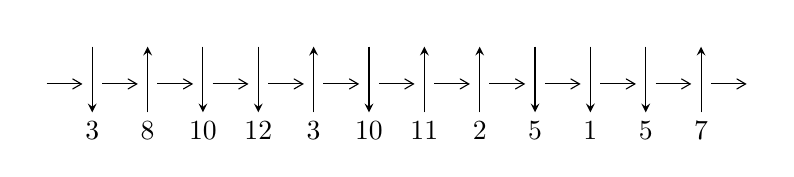
\begin{tikzpicture}[x=20pt, y=17pt]
	% nodes
	\node (C0) at (0, 0) {};
	\node (C1) at (1, 0) {};
	\node (C1U) at (1, +1) {};
	\node (C1D) at (1, -1) {3};

	\node (C2) at (2, 0) {};
	\node (C2U) at (2, +1) {};
	\node (C2D) at (2, -1) {8};

	\node (C3) at (3, 0) {};
	\node (C3U) at (3, +1) {};
	\node (C3D) at (3, -1) {10};

	\node (C4) at (4, 0) {};
	\node (C4U) at (4, +1) {};
	\node (C4D) at (4, -1) {12};

	\node (C5) at (5, 0) {};
	\node (C5U) at (5, +1) {};
	\node (C5D) at (5, -1) {3};

	\node (C6) at (6, 0) {};
	\node (C6U) at (6, +1) {};
	\node (C6D) at (6, -1) {10};

	\node (C7) at (7, 0) {};
	\node (C7U) at (7, +1) {};
	\node (C7D) at (7, -1) {11};

	\node (C8) at (8, 0) {};
	\node (C8U) at (8, +1) {};
	\node (C8D) at (8, -1) {2};

	\node (C9) at (9, 0) {};
	\node (C9U) at (9, +1) {};
	\node (C9D) at (9, -1) {5};

	\node (C10) at (10, 0) {};
	\node (C10U) at (10, +1) {};
	\node (C10D) at (10, -1) {1};

	\node (C11) at (11, 0) {};
	\node (C11U) at (11, +1) {};
	\node (C11D) at (11, -1) {5};

	\node (C12) at (12, 0) {};
	\node (C12U) at (12, +1) {};
	\node (C12D) at (12, -1) {7};
	\node (C13) at (13, 0) {};

	% arrows
	\draw[->,>={angle 60}]
	(C0) edge (C1) (C1) edge (C2) (C2) edge (C3) (C3) edge (C4) (C4) edge (C5) (C5) edge (C6) (C6) edge (C7) (C7) edge (C8) (C8) edge (C9) (C9) edge (C10) (C10) edge (C11) (C11) edge (C12) (C12) edge (C13) ;	\draw[->,>=stealth]
	(C1U) edge (C1D) (C2D) edge (C2U) (C3U) edge (C3D) (C4U) edge (C4D) (C5D) edge (C5U) (C6U) edge (C6D) (C7D) edge (C7U) (C8D) edge (C8U) (C9U) edge (C9D) (C10U) edge (C10D) (C11U) edge (C11D) (C12D) edge (C12U) ;
	\end{tikzpicture} \\
\hhline{~~} \\& 
\textbf{Solving Sequence} \\ \cline{2-2} 
 &
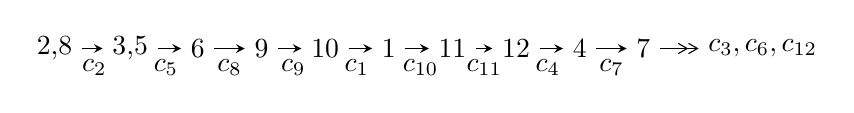
\begin{tikzpicture}[x=23pt, y=7pt]
	% node
	\node (A0) at (-1/8, 0) {2,8};
	\node (A1) at (17/16, 0) {3,5};
	\node (A2) at (17/8, 0) {6};
	\node (A3) at (25/8, 0) {9};
	\node (A4) at (33/8, 0) {10};
	\node (A5) at (41/8, 0) {1};
	\node (A6) at (49/8, 0) {11};
	\node (A7) at (57/8, 0) {12};
	\node (A8) at (65/8, 0) {4};
	\node (A9) at (73/8, 0) {7};
	\node (C1) at (1/2, -1) {$c_{2}$};
	\node (C2) at (13/8, -1) {$c_{5}$};
	\node (C3) at (21/8, -1) {$c_{8}$};
	\node (C4) at (29/8, -1) {$c_{9}$};
	\node (C5) at (37/8, -1) {$c_{1}$};
	\node (C6) at (45/8, -1) {$c_{10}$};
	\node (C7) at (53/8, -1) {$c_{11}$};
	\node (C8) at (61/8, -1) {$c_{4}$};
	\node (C9) at (69/8, -1) {$c_{7}$};
	\node (A10) at (11, 0) {$c_{3},c_{6},c_{12}$};

	% edge
	\draw[->,>=stealth]	
	(A0) edge (A1) (A1) edge (A2) (A2) edge (A3) (A3) edge (A4) (A4) edge (A5) (A5) edge (A6) (A6) edge (A7) (A7) edge (A8) (A8) edge (A9) ;
	\draw[->>,>={angle 60}]	
	(A9) edge (A10);
\end{tikzpicture} \\ 

\end{tabular} \\

\footnotetext{
The image of knot diagram is generated by the software ``\textbf{Draw programme}" developed by Andrew Bartholomew(\url{http://www.layer8.co.uk/maths/draw/index.htm\#Running-draw}), where we modified some parts for our purpose(\url{https://github.com/CATsTAILs/LinksPainter}).
}\phantom \\ \newline 
\centering \textbf{Ideals for irreducible components\footnotemark of $X_{\text{par}}$} 
 
\begin{align*}
I^u_{1}&=\langle 
-1.40561\times10^{133} u^{75}+1.69044\times10^{133} u^{74}+\cdots+6.99960\times10^{133} b-1.41008\times10^{134},\\
\phantom{I^u_{1}}&\phantom{= \langle  }-3.83689\times10^{134} u^{75}+2.93325\times10^{134} u^{74}+\cdots+1.32992\times10^{135} a-2.98368\times10^{136},\\
\phantom{I^u_{1}}&\phantom{= \langle  }u^{76}- u^{75}+\cdots-161 u+38\rangle \\
I^u_{2}&=\langle 
2320203740 u^{35}+625690452 u^{34}+\cdots+215633713 b-4438611716,\\
\phantom{I^u_{2}}&\phantom{= \langle  }18527903408 u^{35}-1296857930 u^{34}+\cdots+1078168565 a-23635723173,\\
\phantom{I^u_{2}}&\phantom{= \langle  }u^{36}+11 u^{34}+\cdots+4 u+5\rangle \\
\\
\end{align*}
\raggedright * 2 irreducible components of $\dim_{\mathbb{C}}=0$, with total 112 representations.\\
\footnotetext{All coefficients of polynomials are rational numbers. But the coefficients are sometimes approximated in decimal forms when there is not enough margin.}
\newpage
\renewcommand{\arraystretch}{1}
\centering \section*{I. $I^u_{1}= \langle -1.41\times10^{133} u^{75}+1.69\times10^{133} u^{74}+\cdots+7.00\times10^{133} b-1.41\times10^{134},\;-3.84\times10^{134} u^{75}+2.93\times10^{134} u^{74}+\cdots+1.33\times10^{135} a-2.98\times10^{136},\;u^{76}- u^{75}+\cdots-161 u+38 \rangle$}
\flushleft \textbf{(i) Arc colorings}\\
\begin{tabular}{m{7pt} m{180pt} m{7pt} m{180pt} }
\flushright $a_{2}=$&$\begin{pmatrix}1\\0\end{pmatrix}$ \\
\flushright $a_{8}=$&$\begin{pmatrix}0\\u\end{pmatrix}$ \\
\flushright $a_{3}=$&$\begin{pmatrix}1\\- u^2\end{pmatrix}$ \\
\flushright $a_{5}=$&$\begin{pmatrix}0.288505 u^{75}-0.220558 u^{74}+\cdots-67.3037 u+22.4350\\0.200813 u^{75}-0.241505 u^{74}+\cdots+2.79038 u+2.01452\end{pmatrix}$ \\
\flushright $a_{6}=$&$\begin{pmatrix}0.343481 u^{75}-0.329454 u^{74}+\cdots-64.5370 u+21.8675\\0.255942 u^{75}-0.347843 u^{74}+\cdots+13.5607 u-0.0344589\end{pmatrix}$ \\
\flushright $a_{9}=$&$\begin{pmatrix}u\\u\end{pmatrix}$ \\
\flushright $a_{10}=$&$\begin{pmatrix}-0.0370385 u^{75}-0.311899 u^{74}+\cdots+197.400 u-40.7028\\0.000948893 u^{75}-0.267585 u^{74}+\cdots+110.531 u-21.4633\end{pmatrix}$ \\
\flushright $a_{1}=$&$\begin{pmatrix}u^2+1\\- u^4\end{pmatrix}$ \\
\flushright $a_{11}=$&$\begin{pmatrix}-0.0506671 u^{75}-0.184581 u^{74}+\cdots+146.321 u-32.9272\\0.0132693 u^{75}-0.287903 u^{74}+\cdots+120.083 u-23.6069\end{pmatrix}$ \\
\flushright $a_{12}=$&$\begin{pmatrix}-0.0878875 u^{75}-0.0853599 u^{74}+\cdots+96.7438 u-15.3384\\-0.0715523 u^{75}-0.214330 u^{74}+\cdots+100.028 u-19.2572\end{pmatrix}$ \\
\flushright $a_{4}=$&$\begin{pmatrix}0.813857 u^{75}-0.422378 u^{74}+\cdots-85.2711 u+45.1346\\-0.0140915 u^{75}+0.246118 u^{74}+\cdots-38.2220 u+11.8442\end{pmatrix}$ \\
\flushright $a_{7}=$&$\begin{pmatrix}0.974728 u^{75}-1.25970 u^{74}+\cdots+96.9366 u-1.10803\\0.131084 u^{75}-0.0921550 u^{74}+\cdots-48.0650 u+11.8828\end{pmatrix}$\\&\end{tabular}
\flushleft \textbf{(ii) Obstruction class $= -1$}\\~\\
\flushleft \textbf{(iii) Cusp Shapes $= -1.23257 u^{75}+1.09381 u^{74}+\cdots-72.2514 u-13.9195$}\\~\\
\newpage\renewcommand{\arraystretch}{1}
\flushleft \textbf{(iv) u-Polynomials at the component}\newline \\
\begin{tabular}{m{50pt}|m{274pt}}
Crossings & \hspace{64pt}u-Polynomials at each crossing \\
\hline $$\begin{aligned}c_{1}\end{aligned}$$&$\begin{aligned}
&u^{76}+31 u^{75}+\cdots+56539 u+1444
\end{aligned}$\\
\hline $$\begin{aligned}c_{2},c_{8}\end{aligned}$$&$\begin{aligned}
&u^{76}+u^{75}+\cdots+161 u+38
\end{aligned}$\\
\hline $$\begin{aligned}c_{3}\end{aligned}$$&$\begin{aligned}
&u^{76}+u^{75}+\cdots+785435 u+192925
\end{aligned}$\\
\hline $$\begin{aligned}c_{4},c_{11}\end{aligned}$$&$\begin{aligned}
&u^{76}+u^{75}+\cdots+115 u+42
\end{aligned}$\\
\hline $$\begin{aligned}c_{5}\end{aligned}$$&$\begin{aligned}
&u^{76}+7 u^{75}+\cdots-176881 u+193903
\end{aligned}$\\
\hline $$\begin{aligned}c_{6}\end{aligned}$$&$\begin{aligned}
&u^{76}- u^{75}+\cdots-1137222277 u+654834962
\end{aligned}$\\
\hline $$\begin{aligned}c_{7}\end{aligned}$$&$\begin{aligned}
&u^{76}-5 u^{75}+\cdots+1855244 u+7111423
\end{aligned}$\\
\hline $$\begin{aligned}c_{9}\end{aligned}$$&$\begin{aligned}
&u^{76}-2 u^{75}+\cdots-34044488 u+10812743
\end{aligned}$\\
\hline $$\begin{aligned}c_{10}\end{aligned}$$&$\begin{aligned}
&u^{76}-3 u^{75}+\cdots+56 u+493
\end{aligned}$\\
\hline $$\begin{aligned}c_{12}\end{aligned}$$&$\begin{aligned}
&u^{76}+u^{75}+\cdots+4761 u+5283
\end{aligned}$\\
\hline
\end{tabular}\\~\\
\newpage\renewcommand{\arraystretch}{1}
\flushleft \textbf{(v) Riley Polynomials at the component}\newline \\
\begin{tabular}{m{50pt}|m{274pt}}
Crossings & \hspace{64pt}Riley Polynomials at each crossing \\
\hline $$\begin{aligned}c_{1}\end{aligned}$$&$\begin{aligned}
&y^{76}+47 y^{75}+\cdots+79202767 y+2085136
\end{aligned}$\\
\hline $$\begin{aligned}c_{2},c_{8}\end{aligned}$$&$\begin{aligned}
&y^{76}+31 y^{75}+\cdots+56539 y+1444
\end{aligned}$\\
\hline $$\begin{aligned}c_{3}\end{aligned}$$&$\begin{aligned}
&y^{76}+115 y^{75}+\cdots+1105604974175 y+37220055625
\end{aligned}$\\
\hline $$\begin{aligned}c_{4},c_{11}\end{aligned}$$&$\begin{aligned}
&y^{76}+67 y^{75}+\cdots-35821 y+1764
\end{aligned}$\\
\hline $$\begin{aligned}c_{5}\end{aligned}$$&$\begin{aligned}
&y^{76}-109 y^{75}+\cdots-932607366479 y+37598373409
\end{aligned}$\\
\hline $$\begin{aligned}c_{6}\end{aligned}$$&$\begin{aligned}
&y^{76}+65 y^{75}+\cdots-1108270808871508769 y+428808827457541444
\end{aligned}$\\
\hline $$\begin{aligned}c_{7}\end{aligned}$$&$\begin{aligned}
&y^{76}-29 y^{75}+\cdots+889309315939338 y+50572337084929
\end{aligned}$\\
\hline $$\begin{aligned}c_{9}\end{aligned}$$&$\begin{aligned}
&y^{76}+102 y^{75}+\cdots-390748923918910 y+116915411184049
\end{aligned}$\\
\hline $$\begin{aligned}c_{10}\end{aligned}$$&$\begin{aligned}
&y^{76}+9 y^{75}+\cdots+7601882 y+243049
\end{aligned}$\\
\hline $$\begin{aligned}c_{12}\end{aligned}$$&$\begin{aligned}
&y^{76}-19 y^{75}+\cdots+69943869 y+27910089
\end{aligned}$\\
\hline
\end{tabular}\\~\\
\newpage\flushleft \textbf{(vi) Complex Volumes and Cusp Shapes}
$$\begin{array}{c|c|c}  
\text{Solutions to }I^u_{1}& \I (\text{vol} + \sqrt{-1}CS) & \text{Cusp shape}\\
 \hline 
\begin{aligned}
u &= -0.662916 + 0.756274 I \\
a &= \phantom{-}1.101880 + 0.248200 I \\
b &= \phantom{-}0.229350 + 0.324684 I\end{aligned}
 & \phantom{-}1.02372 - 2.77677 I & \phantom{-0.000000 } 0 \\ \hline\begin{aligned}
u &= -0.662916 - 0.756274 I \\
a &= \phantom{-}1.101880 - 0.248200 I \\
b &= \phantom{-}0.229350 - 0.324684 I\end{aligned}
 & \phantom{-}1.02372 + 2.77677 I & \phantom{-0.000000 } 0 \\ \hline\begin{aligned}
u &= \phantom{-}0.285315 + 1.007480 I \\
a &= \phantom{-}0.728498 + 0.040863 I \\
b &= \phantom{-}1.107010 - 0.469266 I\end{aligned}
 & -3.83979 - 0.17827 I & \phantom{-0.000000 } 0 \\ \hline\begin{aligned}
u &= \phantom{-}0.285315 - 1.007480 I \\
a &= \phantom{-}0.728498 - 0.040863 I \\
b &= \phantom{-}1.107010 + 0.469266 I\end{aligned}
 & -3.83979 + 0.17827 I & \phantom{-0.000000 } 0 \\ \hline\begin{aligned}
u &= -0.071981 + 0.942071 I \\
a &= \phantom{-}0.052219 + 0.419552 I \\
b &= \phantom{-}1.53394 + 0.19750 I\end{aligned}
 & \phantom{-}6.94756 - 2.68529 I & \phantom{-0.000000 } 0 \\ \hline\begin{aligned}
u &= -0.071981 - 0.942071 I \\
a &= \phantom{-}0.052219 - 0.419552 I \\
b &= \phantom{-}1.53394 - 0.19750 I\end{aligned}
 & \phantom{-}6.94756 + 2.68529 I & \phantom{-0.000000 } 0 \\ \hline\begin{aligned}
u &= -0.801402 + 0.483212 I \\
a &= -0.345937 + 0.673423 I \\
b &= -0.798367 - 0.407778 I\end{aligned}
 & \phantom{-}5.31701 + 1.69426 I & \phantom{-0.000000 } 0 \\ \hline\begin{aligned}
u &= -0.801402 - 0.483212 I \\
a &= -0.345937 - 0.673423 I \\
b &= -0.798367 + 0.407778 I\end{aligned}
 & \phantom{-}5.31701 - 1.69426 I & \phantom{-0.000000 } 0 \\ \hline\begin{aligned}
u &= \phantom{-}0.454063 + 0.966732 I \\
a &= -0.395209 - 1.081370 I \\
b &= -0.834241 - 0.233761 I\end{aligned}
 & -4.65855 + 2.75852 I & \phantom{-0.000000 } 0 \\ \hline\begin{aligned}
u &= \phantom{-}0.454063 - 0.966732 I \\
a &= -0.395209 + 1.081370 I \\
b &= -0.834241 + 0.233761 I\end{aligned}
 & -4.65855 - 2.75852 I & \phantom{-0.000000 } 0\\
 \hline 
 \end{array}$$\newpage$$\begin{array}{c|c|c}  
\text{Solutions to }I^u_{1}& \I (\text{vol} + \sqrt{-1}CS) & \text{Cusp shape}\\
 \hline 
\begin{aligned}
u &= -0.065746 + 1.066650 I \\
a &= \phantom{-}0.553908 - 0.016598 I \\
b &= \phantom{-}0.004846 + 0.584532 I\end{aligned}
 & -0.0217467 + 0.0606793 I & \phantom{-0.000000 } 0 \\ \hline\begin{aligned}
u &= -0.065746 - 1.066650 I \\
a &= \phantom{-}0.553908 + 0.016598 I \\
b &= \phantom{-}0.004846 - 0.584532 I\end{aligned}
 & -0.0217467 - 0.0606793 I & \phantom{-0.000000 } 0 \\ \hline\begin{aligned}
u &= \phantom{-}0.817443 + 0.712232 I \\
a &= -1.65495 + 1.01142 I \\
b &= -0.80510 + 2.04740 I\end{aligned}
 & \phantom{-}7.26372 + 0.80285 I & \phantom{-0.000000 } 0 \\ \hline\begin{aligned}
u &= \phantom{-}0.817443 - 0.712232 I \\
a &= -1.65495 - 1.01142 I \\
b &= -0.80510 - 2.04740 I\end{aligned}
 & \phantom{-}7.26372 - 0.80285 I & \phantom{-0.000000 } 0 \\ \hline\begin{aligned}
u &= -0.567079 + 0.930252 I \\
a &= \phantom{-}0.286387 + 0.362192 I \\
b &= \phantom{-}0.304274 + 0.981241 I\end{aligned}
 & \phantom{-}0.45994 - 2.05238 I & \phantom{-0.000000 } 0 \\ \hline\begin{aligned}
u &= -0.567079 - 0.930252 I \\
a &= \phantom{-}0.286387 - 0.362192 I \\
b &= \phantom{-}0.304274 - 0.981241 I\end{aligned}
 & \phantom{-}0.45994 + 2.05238 I & \phantom{-0.000000 } 0 \\ \hline\begin{aligned}
u &= -0.035983 + 0.897156 I \\
a &= \phantom{-}1.98195 + 0.37899 I \\
b &= \phantom{-}1.39142 + 1.28975 I\end{aligned}
 & -0.86327 - 4.72694 I & \phantom{-0.000000 -}0. + 5.69238 I \\ \hline\begin{aligned}
u &= -0.035983 - 0.897156 I \\
a &= \phantom{-}1.98195 - 0.37899 I \\
b &= \phantom{-}1.39142 - 1.28975 I\end{aligned}
 & -0.86327 + 4.72694 I & \phantom{-0.000000 } 0. - 5.69238 I \\ \hline\begin{aligned}
u &= -0.776192 + 0.835014 I \\
a &= \phantom{-}2.07774 + 1.16141 I \\
b &= \phantom{-}0.77380 + 2.17827 I\end{aligned}
 & \phantom{-}11.69860 - 4.05347 I & \phantom{-0.000000 } 0 \\ \hline\begin{aligned}
u &= -0.776192 - 0.835014 I \\
a &= \phantom{-}2.07774 - 1.16141 I \\
b &= \phantom{-}0.77380 - 2.17827 I\end{aligned}
 & \phantom{-}11.69860 + 4.05347 I & \phantom{-0.000000 } 0\\
 \hline 
 \end{array}$$\newpage$$\begin{array}{c|c|c}  
\text{Solutions to }I^u_{1}& \I (\text{vol} + \sqrt{-1}CS) & \text{Cusp shape}\\
 \hline 
\begin{aligned}
u &= \phantom{-}0.685008 + 0.481376 I \\
a &= -0.671350 + 0.806633 I \\
b &= -0.324604 + 0.807985 I\end{aligned}
 & \phantom{-}5.03216 - 1.01780 I & \phantom{-}3.86360 + 0.75310 I \\ \hline\begin{aligned}
u &= \phantom{-}0.685008 - 0.481376 I \\
a &= -0.671350 - 0.806633 I \\
b &= -0.324604 - 0.807985 I\end{aligned}
 & \phantom{-}5.03216 + 1.01780 I & \phantom{-}3.86360 - 0.75310 I \\ \hline\begin{aligned}
u &= \phantom{-}0.674753 + 0.493249 I \\
a &= \phantom{-}0.892957 - 0.164512 I \\
b &= -0.0532868 + 0.0446471 I\end{aligned}
 & \phantom{-}0.03629 - 1.91884 I & -4.55374 + 4.02239 I \\ \hline\begin{aligned}
u &= \phantom{-}0.674753 - 0.493249 I \\
a &= \phantom{-}0.892957 + 0.164512 I \\
b &= -0.0532868 - 0.0446471 I\end{aligned}
 & \phantom{-}0.03629 + 1.91884 I & -4.55374 - 4.02239 I \\ \hline\begin{aligned}
u &= \phantom{-}0.125956 + 1.164950 I \\
a &= \phantom{-}0.793952 + 0.447911 I \\
b &= -0.331670 + 0.408432 I\end{aligned}
 & \phantom{-}1.57754 + 1.96619 I & \phantom{-0.000000 } 0 \\ \hline\begin{aligned}
u &= \phantom{-}0.125956 - 1.164950 I \\
a &= \phantom{-}0.793952 - 0.447911 I \\
b &= -0.331670 - 0.408432 I\end{aligned}
 & \phantom{-}1.57754 - 1.96619 I & \phantom{-0.000000 } 0 \\ \hline\begin{aligned}
u &= -0.905570 + 0.746388 I \\
a &= -1.56681 - 0.61842 I \\
b &= -0.60049 - 2.22973 I\end{aligned}
 & \phantom{-}9.01118 + 2.11338 I & \phantom{-0.000000 } 0 \\ \hline\begin{aligned}
u &= -0.905570 - 0.746388 I \\
a &= -1.56681 + 0.61842 I \\
b &= -0.60049 + 2.22973 I\end{aligned}
 & \phantom{-}9.01118 - 2.11338 I & \phantom{-0.000000 } 0 \\ \hline\begin{aligned}
u &= \phantom{-}0.857518 + 0.845288 I \\
a &= \phantom{-}1.71489 - 1.10425 I \\
b &= \phantom{-}0.03590 - 2.23093 I\end{aligned}
 & \phantom{-}13.33450 - 0.74413 I & \phantom{-0.000000 } 0 \\ \hline\begin{aligned}
u &= \phantom{-}0.857518 - 0.845288 I \\
a &= \phantom{-}1.71489 + 1.10425 I \\
b &= \phantom{-}0.03590 + 2.23093 I\end{aligned}
 & \phantom{-}13.33450 + 0.74413 I & \phantom{-0.000000 } 0\\
 \hline 
 \end{array}$$\newpage$$\begin{array}{c|c|c}  
\text{Solutions to }I^u_{1}& \I (\text{vol} + \sqrt{-1}CS) & \text{Cusp shape}\\
 \hline 
\begin{aligned}
u &= \phantom{-}0.808599 + 0.893250 I \\
a &= -1.48978 + 0.39296 I \\
b &= -0.695470 + 0.566481 I\end{aligned}
 & \phantom{-}4.03943 + 7.86346 I & \phantom{-0.000000 } 0 \\ \hline\begin{aligned}
u &= \phantom{-}0.808599 - 0.893250 I \\
a &= -1.48978 - 0.39296 I \\
b &= -0.695470 - 0.566481 I\end{aligned}
 & \phantom{-}4.03943 - 7.86346 I & \phantom{-0.000000 } 0 \\ \hline\begin{aligned}
u &= -0.755392 + 0.942068 I \\
a &= \phantom{-}1.35234 + 1.51692 I \\
b &= \phantom{-}0.40854 + 2.69108 I\end{aligned}
 & \phantom{-}11.36750 - 1.74590 I & \phantom{-0.000000 } 0 \\ \hline\begin{aligned}
u &= -0.755392 - 0.942068 I \\
a &= \phantom{-}1.35234 - 1.51692 I \\
b &= \phantom{-}0.40854 - 2.69108 I\end{aligned}
 & \phantom{-}11.36750 + 1.74590 I & \phantom{-0.000000 } 0 \\ \hline\begin{aligned}
u &= \phantom{-}0.586707 + 1.057010 I \\
a &= -0.847409 + 0.771102 I \\
b &= -0.574387 + 1.013170 I\end{aligned}
 & \phantom{-}3.36226 + 5.96102 I & \phantom{-0.000000 } 0 \\ \hline\begin{aligned}
u &= \phantom{-}0.586707 - 1.057010 I \\
a &= -0.847409 - 0.771102 I \\
b &= -0.574387 - 1.013170 I\end{aligned}
 & \phantom{-}3.36226 - 5.96102 I & \phantom{-0.000000 } 0 \\ \hline\begin{aligned}
u &= -0.891731 + 0.840665 I \\
a &= -0.481551 + 0.251785 I \\
b &= -1.12694 - 1.25772 I\end{aligned}
 & \phantom{-}5.26607 - 5.97794 I & \phantom{-0.000000 } 0 \\ \hline\begin{aligned}
u &= -0.891731 - 0.840665 I \\
a &= -0.481551 - 0.251785 I \\
b &= -1.12694 + 1.25772 I\end{aligned}
 & \phantom{-}5.26607 + 5.97794 I & \phantom{-0.000000 } 0 \\ \hline\begin{aligned}
u &= \phantom{-}0.586220 + 1.081390 I \\
a &= \phantom{-}0.133904 - 0.312139 I \\
b &= \phantom{-}0.300788 - 0.900121 I\end{aligned}
 & -1.72755 + 6.88426 I & \phantom{-0.000000 } 0 \\ \hline\begin{aligned}
u &= \phantom{-}0.586220 - 1.081390 I \\
a &= \phantom{-}0.133904 + 0.312139 I \\
b &= \phantom{-}0.300788 + 0.900121 I\end{aligned}
 & -1.72755 - 6.88426 I & \phantom{-0.000000 } 0\\
 \hline 
 \end{array}$$\newpage$$\begin{array}{c|c|c}  
\text{Solutions to }I^u_{1}& \I (\text{vol} + \sqrt{-1}CS) & \text{Cusp shape}\\
 \hline 
\begin{aligned}
u &= \phantom{-}0.833867 + 0.931666 I \\
a &= \phantom{-}0.011648 + 0.675666 I \\
b &= -0.22419 + 1.43475 I\end{aligned}
 & \phantom{-}3.94945 - 1.73029 I & \phantom{-0.000000 } 0 \\ \hline\begin{aligned}
u &= \phantom{-}0.833867 - 0.931666 I \\
a &= \phantom{-}0.011648 - 0.675666 I \\
b &= -0.22419 - 1.43475 I\end{aligned}
 & \phantom{-}3.94945 + 1.73029 I & \phantom{-0.000000 } 0 \\ \hline\begin{aligned}
u &= -0.620183 + 1.088800 I \\
a &= \phantom{-}0.271097 - 0.813299 I \\
b &= \phantom{-}1.066280 - 0.583822 I\end{aligned}
 & \phantom{-}3.47667 - 7.03715 I & \phantom{-0.000000 } 0 \\ \hline\begin{aligned}
u &= -0.620183 - 1.088800 I \\
a &= \phantom{-}0.271097 + 0.813299 I \\
b &= \phantom{-}1.066280 + 0.583822 I\end{aligned}
 & \phantom{-}3.47667 + 7.03715 I & \phantom{-0.000000 } 0 \\ \hline\begin{aligned}
u &= \phantom{-}0.812966 + 0.968903 I \\
a &= \phantom{-}1.47513 - 1.02155 I \\
b &= \phantom{-}0.60131 - 2.65223 I\end{aligned}
 & \phantom{-}12.9447 + 6.9741 I & \phantom{-0.000000 } 0 \\ \hline\begin{aligned}
u &= \phantom{-}0.812966 - 0.968903 I \\
a &= \phantom{-}1.47513 + 1.02155 I \\
b &= \phantom{-}0.60131 + 2.65223 I\end{aligned}
 & \phantom{-}12.9447 - 6.9741 I & \phantom{-0.000000 } 0 \\ \hline\begin{aligned}
u &= \phantom{-}0.417255 + 0.595574 I \\
a &= \phantom{-}0.906862 + 1.028830 I \\
b &= \phantom{-}1.44318 - 0.59225 I\end{aligned}
 & -3.48958 + 0.81926 I & -1.10723 + 7.17810 I \\ \hline\begin{aligned}
u &= \phantom{-}0.417255 - 0.595574 I \\
a &= \phantom{-}0.906862 - 1.028830 I \\
b &= \phantom{-}1.44318 + 0.59225 I\end{aligned}
 & -3.48958 - 0.81926 I & -1.10723 - 7.17810 I \\ \hline\begin{aligned}
u &= \phantom{-}0.755325 + 1.024620 I \\
a &= -1.47153 + 1.42806 I \\
b &= -0.57159 + 2.27179 I\end{aligned}
 & \phantom{-}6.31700 + 5.12272 I & \phantom{-0.000000 } 0 \\ \hline\begin{aligned}
u &= \phantom{-}0.755325 - 1.024620 I \\
a &= -1.47153 - 1.42806 I \\
b &= -0.57159 - 2.27179 I\end{aligned}
 & \phantom{-}6.31700 - 5.12272 I & \phantom{-0.000000 } 0\\
 \hline 
 \end{array}$$\newpage$$\begin{array}{c|c|c}  
\text{Solutions to }I^u_{1}& \I (\text{vol} + \sqrt{-1}CS) & \text{Cusp shape}\\
 \hline 
\begin{aligned}
u &= \phantom{-}1.122970 + 0.615953 I \\
a &= \phantom{-}1.43503 - 0.45100 I \\
b &= \phantom{-}0.21012 - 1.85984 I\end{aligned}
 & \phantom{-}15.5887 - 9.4779 I & \phantom{-0.000000 } 0 \\ \hline\begin{aligned}
u &= \phantom{-}1.122970 - 0.615953 I \\
a &= \phantom{-}1.43503 + 0.45100 I \\
b &= \phantom{-}0.21012 + 1.85984 I\end{aligned}
 & \phantom{-}15.5887 + 9.4779 I & \phantom{-0.000000 } 0 \\ \hline\begin{aligned}
u &= -0.097362 + 0.683736 I \\
a &= -2.21326 + 0.89923 I \\
b &= \phantom{-}0.083644 + 0.547260 I\end{aligned}
 & \phantom{-}8.06044 + 1.96087 I & -6.97401 - 6.64687 I \\ \hline\begin{aligned}
u &= -0.097362 - 0.683736 I \\
a &= -2.21326 - 0.89923 I \\
b &= \phantom{-}0.083644 - 0.547260 I\end{aligned}
 & \phantom{-}8.06044 - 1.96087 I & -6.97401 + 6.64687 I \\ \hline\begin{aligned}
u &= -0.793679 + 1.042660 I \\
a &= -1.39866 - 1.40506 I \\
b &= -0.07618 - 2.49555 I\end{aligned}
 & \phantom{-}8.08586 - 8.41406 I & \phantom{-0.000000 } 0 \\ \hline\begin{aligned}
u &= -0.793679 - 1.042660 I \\
a &= -1.39866 + 1.40506 I \\
b &= -0.07618 + 2.49555 I\end{aligned}
 & \phantom{-}8.08586 + 8.41406 I & \phantom{-0.000000 } 0 \\ \hline\begin{aligned}
u &= \phantom{-}0.143179 + 0.668479 I \\
a &= -2.73389 + 1.26855 I \\
b &= -1.91204 + 0.24981 I\end{aligned}
 & \phantom{-}0.07264 + 5.18640 I & -2.24311 - 3.02074 I \\ \hline\begin{aligned}
u &= \phantom{-}0.143179 - 0.668479 I \\
a &= -2.73389 - 1.26855 I \\
b &= -1.91204 - 0.24981 I\end{aligned}
 & \phantom{-}0.07264 - 5.18640 I & -2.24311 + 3.02074 I \\ \hline\begin{aligned}
u &= -0.868591 + 1.008050 I \\
a &= -0.612283 - 0.762405 I \\
b &= \phantom{-}0.798677 - 0.486252 I\end{aligned}
 & \phantom{-}4.77438 - 0.52879 I & \phantom{-0.000000 } 0 \\ \hline\begin{aligned}
u &= -0.868591 - 1.008050 I \\
a &= -0.612283 + 0.762405 I \\
b &= \phantom{-}0.798677 + 0.486252 I\end{aligned}
 & \phantom{-}4.77438 + 0.52879 I & \phantom{-0.000000 } 0\\
 \hline 
 \end{array}$$\newpage$$\begin{array}{c|c|c}  
\text{Solutions to }I^u_{1}& \I (\text{vol} + \sqrt{-1}CS) & \text{Cusp shape}\\
 \hline 
\begin{aligned}
u &= -1.281600 + 0.509659 I \\
a &= \phantom{-}1.165520 + 0.192564 I \\
b &= \phantom{-}0.15176 + 1.69413 I\end{aligned}
 & \phantom{-}14.2247 - 0.6780 I & \phantom{-0.000000 } 0 \\ \hline\begin{aligned}
u &= -1.281600 - 0.509659 I \\
a &= \phantom{-}1.165520 - 0.192564 I \\
b &= \phantom{-}0.15176 - 1.69413 I\end{aligned}
 & \phantom{-}14.2247 + 0.6780 I & \phantom{-0.000000 } 0 \\ \hline\begin{aligned}
u &= \phantom{-}0.80610 + 1.17936 I \\
a &= \phantom{-}1.10730 - 1.40702 I \\
b &= \phantom{-}0.16133 - 2.68309 I\end{aligned}
 & \phantom{-}13.7755 + 16.3958 I & \phantom{-0.000000 } 0 \\ \hline\begin{aligned}
u &= \phantom{-}0.80610 - 1.17936 I \\
a &= \phantom{-}1.10730 + 1.40702 I \\
b &= \phantom{-}0.16133 + 2.68309 I\end{aligned}
 & \phantom{-}13.7755 - 16.3958 I & \phantom{-0.000000 } 0 \\ \hline\begin{aligned}
u &= -0.211361 + 0.486832 I \\
a &= \phantom{-}0.397591 - 0.482624 I \\
b &= -0.064564 + 0.403505 I\end{aligned}
 & -0.073057 - 1.023140 I & -1.34729 + 6.93509 I \\ \hline\begin{aligned}
u &= -0.211361 - 0.486832 I \\
a &= \phantom{-}0.397591 + 0.482624 I \\
b &= -0.064564 - 0.403505 I\end{aligned}
 & -0.073057 + 1.023140 I & -1.34729 - 6.93509 I \\ \hline\begin{aligned}
u &= -0.071583 + 0.511345 I \\
a &= -3.10512 - 1.44557 I \\
b &= -1.297630 - 0.234701 I\end{aligned}
 & -1.77992 + 1.19696 I & \phantom{-}0.03557 + 2.38161 I \\ \hline\begin{aligned}
u &= -0.071583 - 0.511345 I \\
a &= -3.10512 + 1.44557 I \\
b &= -1.297630 + 0.234701 I\end{aligned}
 & -1.77992 - 1.19696 I & \phantom{-}0.03557 - 2.38161 I \\ \hline\begin{aligned}
u &= \phantom{-}0.01963 + 1.54289 I \\
a &= \phantom{-}0.20427 - 1.41812 I \\
b &= \phantom{-}0.06304 - 2.22995 I\end{aligned}
 & -6.31186 - 1.00322 I & \phantom{-0.000000 } 0 \\ \hline\begin{aligned}
u &= \phantom{-}0.01963 - 1.54289 I \\
a &= \phantom{-}0.20427 + 1.41812 I \\
b &= \phantom{-}0.06304 + 2.22995 I\end{aligned}
 & -6.31186 + 1.00322 I & \phantom{-0.000000 } 0\\
 \hline 
 \end{array}$$\newpage$$\begin{array}{c|c|c}  
\text{Solutions to }I^u_{1}& \I (\text{vol} + \sqrt{-1}CS) & \text{Cusp shape}\\
 \hline 
\begin{aligned}
u &= -0.85412 + 1.28528 I \\
a &= \phantom{-}0.84162 + 1.24436 I \\
b &= -0.09692 + 2.44856 I\end{aligned}
 & \phantom{-}11.80170 - 6.84042 I & \phantom{-0.000000 } 0 \\ \hline\begin{aligned}
u &= -0.85412 - 1.28528 I \\
a &= \phantom{-}0.84162 - 1.24436 I \\
b &= -0.09692 - 2.44856 I\end{aligned}
 & \phantom{-}11.80170 + 6.84042 I & \phantom{-0.000000 } 0 \\ \hline\begin{aligned}
u &= -0.17757 + 1.56950 I \\
a &= -0.345899 - 0.007011 I \\
b &= \phantom{-}1.013900 - 0.055144 I\end{aligned}
 & \phantom{-}6.48446 - 6.01294 I & \phantom{-0.000000 } 0 \\ \hline\begin{aligned}
u &= -0.17757 - 1.56950 I \\
a &= -0.345899 + 0.007011 I \\
b &= \phantom{-}1.013900 + 0.055144 I\end{aligned}
 & \phantom{-}6.48446 + 6.01294 I & \phantom{-0.000000 } 0 \\ \hline\begin{aligned}
u &= \phantom{-}0.217162 + 0.333065 I \\
a &= -0.21882 + 2.01262 I \\
b &= -1.295440 + 0.442525 I\end{aligned}
 & \phantom{-}5.12456 - 0.63054 I & \phantom{-}2.98724 - 1.55101 I \\ \hline\begin{aligned}
u &= \phantom{-}0.217162 - 0.333065 I \\
a &= -0.21882 - 2.01262 I \\
b &= -1.295440 - 0.442525 I\end{aligned}
 & \phantom{-}5.12456 + 0.63054 I & \phantom{-}2.98724 + 1.55101 I\\
 \hline 
 \end{array}$$\newpage\newpage\renewcommand{\arraystretch}{1}
\centering \section*{II. $I^u_{2}= \langle 2.32\times10^{9} u^{35}+6.26\times10^{8} u^{34}+\cdots+2.16\times10^{8} b-4.44\times10^{9},\;1.85\times10^{10} u^{35}-1.30\times10^{9} u^{34}+\cdots+1.08\times10^{9} a-2.36\times10^{10},\;u^{36}+11 u^{34}+\cdots+4 u+5 \rangle$}
\flushleft \textbf{(i) Arc colorings}\\
\begin{tabular}{m{7pt} m{180pt} m{7pt} m{180pt} }
\flushright $a_{2}=$&$\begin{pmatrix}1\\0\end{pmatrix}$ \\
\flushright $a_{8}=$&$\begin{pmatrix}0\\u\end{pmatrix}$ \\
\flushright $a_{3}=$&$\begin{pmatrix}1\\- u^2\end{pmatrix}$ \\
\flushright $a_{5}=$&$\begin{pmatrix}-17.1846 u^{35}+1.20283 u^{34}+\cdots-75.7116 u+21.9221\\-10.7599 u^{35}-2.90164 u^{34}+\cdots-25.2606 u+20.5840\end{pmatrix}$ \\
\flushright $a_{6}=$&$\begin{pmatrix}-16.6658 u^{35}+2.34552 u^{34}+\cdots-19.8606 u+36.4920\\-14.2879 u^{35}-3.75044 u^{34}+\cdots-18.0959 u+26.2975\end{pmatrix}$ \\
\flushright $a_{9}=$&$\begin{pmatrix}u\\u\end{pmatrix}$ \\
\flushright $a_{10}=$&$\begin{pmatrix}3.12153 u^{35}+3.61119 u^{34}+\cdots+51.1214 u+40.2398\\-2.89850 u^{35}+1.59421 u^{34}+\cdots+4.90691 u-0.328315\end{pmatrix}$ \\
\flushright $a_{1}=$&$\begin{pmatrix}u^2+1\\- u^4\end{pmatrix}$ \\
\flushright $a_{11}=$&$\begin{pmatrix}1.64216 u^{35}+3.57318 u^{34}+\cdots+27.8545 u+41.5188\\-5.57167 u^{35}-0.0804230 u^{34}+\cdots-16.1199 u-6.11863\end{pmatrix}$ \\
\flushright $a_{12}=$&$\begin{pmatrix}-1.64253 u^{35}-7.92125 u^{34}+\cdots-93.3783 u+4.52924\\-5.74240 u^{35}-12.0937 u^{34}+\cdots-135.508 u-86.5034\end{pmatrix}$ \\
\flushright $a_{4}=$&$\begin{pmatrix}18.3632 u^{35}-6.24544 u^{34}+\cdots+113.684 u-33.6728\\5.42696 u^{35}+5.48132 u^{34}+\cdots-2.11327 u+26.8602\end{pmatrix}$ \\
\flushright $a_{7}=$&$\begin{pmatrix}-6.20362 u^{35}-12.5212 u^{34}+\cdots+8.52928 u-73.1894\\-7.13644 u^{35}-6.41854 u^{34}+\cdots-49.4761 u+11.3475\end{pmatrix}$\\&\end{tabular}
\flushleft \textbf{(ii) Obstruction class $= 1$}\\~\\
\flushleft \textbf{(iii) Cusp Shapes $= \frac{4184661271}{215633713} u^{35}-\frac{680860653}{215633713} u^{34}+\cdots+\frac{99258781362}{215633713} u+\frac{14533752217}{215633713}$}\\~\\
\newpage\renewcommand{\arraystretch}{1}
\flushleft \textbf{(iv) u-Polynomials at the component}\newline \\
\begin{tabular}{m{50pt}|m{274pt}}
Crossings & \hspace{64pt}u-Polynomials at each crossing \\
\hline $$\begin{aligned}c_{1}\end{aligned}$$&$\begin{aligned}
&u^{36}-22 u^{35}+\cdots-464 u+25
\end{aligned}$\\
\hline $$\begin{aligned}c_{2}\end{aligned}$$&$\begin{aligned}
&u^{36}+11 u^{34}+\cdots+4 u+5
\end{aligned}$\\
\hline $$\begin{aligned}c_{3}\end{aligned}$$&$\begin{aligned}
&u^{36}+19 u^{34}+\cdots-435 u+493
\end{aligned}$\\
\hline $$\begin{aligned}c_{4}\end{aligned}$$&$\begin{aligned}
&u^{36}+11 u^{34}+\cdots+4 u+5
\end{aligned}$\\
\hline $$\begin{aligned}c_{5}\end{aligned}$$&$\begin{aligned}
&u^{36}-14 u^{35}+\cdots-973 u+73
\end{aligned}$\\
\hline $$\begin{aligned}c_{6}\end{aligned}$$&$\begin{aligned}
&u^{36}+2 u^{35}+\cdots+1163 u+175
\end{aligned}$\\
\hline $$\begin{aligned}c_{7}\end{aligned}$$&$\begin{aligned}
&u^{36}+3 u^{34}+\cdots-82 u+29
\end{aligned}$\\
\hline $$\begin{aligned}c_{8}\end{aligned}$$&$\begin{aligned}
&u^{36}+11 u^{34}+\cdots-4 u+5
\end{aligned}$\\
\hline $$\begin{aligned}c_{9}\end{aligned}$$&$\begin{aligned}
&u^{36}+u^{35}+\cdots-2 u+1
\end{aligned}$\\
\hline $$\begin{aligned}c_{10}\end{aligned}$$&$\begin{aligned}
&u^{36}-6 u^{35}+\cdots+2 u+1
\end{aligned}$\\
\hline $$\begin{aligned}c_{11}\end{aligned}$$&$\begin{aligned}
&u^{36}+11 u^{34}+\cdots-4 u+5
\end{aligned}$\\
\hline $$\begin{aligned}c_{12}\end{aligned}$$&$\begin{aligned}
&u^{36}+2 u^{34}+\cdots- u+1
\end{aligned}$\\
\hline
\end{tabular}\\~\\
\newpage\renewcommand{\arraystretch}{1}
\flushleft \textbf{(v) Riley Polynomials at the component}\newline \\
\begin{tabular}{m{50pt}|m{274pt}}
Crossings & \hspace{64pt}Riley Polynomials at each crossing \\
\hline $$\begin{aligned}c_{1}\end{aligned}$$&$\begin{aligned}
&y^{36}+2 y^{35}+\cdots+804 y+625
\end{aligned}$\\
\hline $$\begin{aligned}c_{2},c_{8}\end{aligned}$$&$\begin{aligned}
&y^{36}+22 y^{35}+\cdots+464 y+25
\end{aligned}$\\
\hline $$\begin{aligned}c_{3}\end{aligned}$$&$\begin{aligned}
&y^{36}+38 y^{35}+\cdots+3007387 y+243049
\end{aligned}$\\
\hline $$\begin{aligned}c_{4},c_{11}\end{aligned}$$&$\begin{aligned}
&y^{36}+22 y^{35}+\cdots+564 y+25
\end{aligned}$\\
\hline $$\begin{aligned}c_{5}\end{aligned}$$&$\begin{aligned}
&y^{36}-38 y^{35}+\cdots-246659 y+5329
\end{aligned}$\\
\hline $$\begin{aligned}c_{6}\end{aligned}$$&$\begin{aligned}
&y^{36}+20 y^{35}+\cdots+89081 y+30625
\end{aligned}$\\
\hline $$\begin{aligned}c_{7}\end{aligned}$$&$\begin{aligned}
&y^{36}+6 y^{35}+\cdots+33006 y+841
\end{aligned}$\\
\hline $$\begin{aligned}c_{9}\end{aligned}$$&$\begin{aligned}
&y^{36}+13 y^{35}+\cdots-18 y+1
\end{aligned}$\\
\hline $$\begin{aligned}c_{10}\end{aligned}$$&$\begin{aligned}
&y^{36}-8 y^{35}+\cdots+30 y+1
\end{aligned}$\\
\hline $$\begin{aligned}c_{12}\end{aligned}$$&$\begin{aligned}
&y^{36}+4 y^{35}+\cdots-27 y+1
\end{aligned}$\\
\hline
\end{tabular}\\~\\
\newpage\flushleft \textbf{(vi) Complex Volumes and Cusp Shapes}
$$\begin{array}{c|c|c}  
\text{Solutions to }I^u_{2}& \I (\text{vol} + \sqrt{-1}CS) & \text{Cusp shape}\\
 \hline 
\begin{aligned}
u &= \phantom{-}0.346186 + 0.915633 I \\
a &= -2.18981 + 0.04924 I \\
b &= -2.30967 + 0.67789 I\end{aligned}
 & -0.09061 + 6.29545 I & -2.74141 - 9.81893 I \\ \hline\begin{aligned}
u &= \phantom{-}0.346186 - 0.915633 I \\
a &= -2.18981 - 0.04924 I \\
b &= -2.30967 - 0.67789 I\end{aligned}
 & -0.09061 - 6.29545 I & -2.74141 + 9.81893 I \\ \hline\begin{aligned}
u &= \phantom{-}0.358539 + 0.889505 I \\
a &= \phantom{-}1.10628 + 1.99818 I \\
b &= \phantom{-}1.35666 + 1.39465 I\end{aligned}
 & -0.01798 - 3.35229 I & -0.148269 + 0.744013 I \\ \hline\begin{aligned}
u &= \phantom{-}0.358539 - 0.889505 I \\
a &= \phantom{-}1.10628 - 1.99818 I \\
b &= \phantom{-}1.35666 - 1.39465 I\end{aligned}
 & -0.01798 + 3.35229 I & -0.148269 - 0.744013 I \\ \hline\begin{aligned}
u &= \phantom{-}0.793225 + 0.705083 I \\
a &= \phantom{-}0.175649 + 0.251827 I \\
b &= -0.443614 + 0.878255 I\end{aligned}
 & \phantom{-}2.93798 - 2.72322 I & -0.38581 + 3.76403 I \\ \hline\begin{aligned}
u &= \phantom{-}0.793225 - 0.705083 I \\
a &= \phantom{-}0.175649 - 0.251827 I \\
b &= -0.443614 - 0.878255 I\end{aligned}
 & \phantom{-}2.93798 + 2.72322 I & -0.38581 - 3.76403 I \\ \hline\begin{aligned}
u &= -0.833697 + 0.409348 I \\
a &= -0.992290 - 0.210555 I \\
b &= -0.204707 + 0.035403 I\end{aligned}
 & \phantom{-}1.05225 + 1.68422 I & \phantom{-}3.81700 - 1.49163 I \\ \hline\begin{aligned}
u &= -0.833697 - 0.409348 I \\
a &= -0.992290 + 0.210555 I \\
b &= -0.204707 - 0.035403 I\end{aligned}
 & \phantom{-}1.05225 - 1.68422 I & \phantom{-}3.81700 + 1.49163 I \\ \hline\begin{aligned}
u &= \phantom{-}0.791352 + 0.733206 I \\
a &= -1.47082 + 1.03484 I \\
b &= -0.79762 + 2.14988 I\end{aligned}
 & \phantom{-}7.23477 + 0.01514 I & \phantom{-}3.93034 + 2.41109 I \\ \hline\begin{aligned}
u &= \phantom{-}0.791352 - 0.733206 I \\
a &= -1.47082 - 1.03484 I \\
b &= -0.79762 - 2.14988 I\end{aligned}
 & \phantom{-}7.23477 - 0.01514 I & \phantom{-}3.93034 - 2.41109 I\\
 \hline 
 \end{array}$$\newpage$$\begin{array}{c|c|c}  
\text{Solutions to }I^u_{2}& \I (\text{vol} + \sqrt{-1}CS) & \text{Cusp shape}\\
 \hline 
\begin{aligned}
u &= -0.485657 + 0.963636 I \\
a &= -0.330010 + 1.341270 I \\
b &= -0.897778 + 0.513044 I\end{aligned}
 & -4.27615 - 2.65956 I & \phantom{-}5.82571 + 1.68378 I \\ \hline\begin{aligned}
u &= -0.485657 - 0.963636 I \\
a &= -0.330010 - 1.341270 I \\
b &= -0.897778 - 0.513044 I\end{aligned}
 & -4.27615 + 2.65956 I & \phantom{-}5.82571 - 1.68378 I \\ \hline\begin{aligned}
u &= -0.295770 + 1.046740 I \\
a &= -0.668520 - 0.246425 I \\
b &= -1.196780 - 0.522064 I\end{aligned}
 & -3.40683 - 0.20848 I & -1.58036 + 4.45786 I \\ \hline\begin{aligned}
u &= -0.295770 - 1.046740 I \\
a &= -0.668520 + 0.246425 I \\
b &= -1.196780 + 0.522064 I\end{aligned}
 & -3.40683 + 0.20848 I & -1.58036 - 4.45786 I \\ \hline\begin{aligned}
u &= -0.481168 + 0.730864 I \\
a &= \phantom{-}0.943466 - 0.719816 I \\
b &= \phantom{-}1.54841 + 0.64568 I\end{aligned}
 & -3.47907 - 1.30636 I & -0.49756 + 8.73623 I \\ \hline\begin{aligned}
u &= -0.481168 - 0.730864 I \\
a &= \phantom{-}0.943466 + 0.719816 I \\
b &= \phantom{-}1.54841 - 0.64568 I\end{aligned}
 & -3.47907 + 1.30636 I & -0.49756 - 8.73623 I \\ \hline\begin{aligned}
u &= \phantom{-}0.638782 + 0.989341 I \\
a &= -0.602797 + 0.604049 I \\
b &= -0.147279 + 0.094498 I\end{aligned}
 & \phantom{-}2.02425 + 8.10760 I & -2.00000 - 8.42655 I \\ \hline\begin{aligned}
u &= \phantom{-}0.638782 - 0.989341 I \\
a &= -0.602797 - 0.604049 I \\
b &= -0.147279 - 0.094498 I\end{aligned}
 & \phantom{-}2.02425 - 8.10760 I & -2.00000 + 8.42655 I \\ \hline\begin{aligned}
u &= \phantom{-}0.387249 + 1.117620 I \\
a &= \phantom{-}0.724091 + 0.876891 I \\
b &= \phantom{-}0.040960 + 0.770428 I\end{aligned}
 & \phantom{-}3.07088 + 1.37025 I & \phantom{-}3.22960 - 2.00825 I \\ \hline\begin{aligned}
u &= \phantom{-}0.387249 - 1.117620 I \\
a &= \phantom{-}0.724091 - 0.876891 I \\
b &= \phantom{-}0.040960 - 0.770428 I\end{aligned}
 & \phantom{-}3.07088 - 1.37025 I & \phantom{-}3.22960 + 2.00825 I\\
 \hline 
 \end{array}$$\newpage$$\begin{array}{c|c|c}  
\text{Solutions to }I^u_{2}& \I (\text{vol} + \sqrt{-1}CS) & \text{Cusp shape}\\
 \hline 
\begin{aligned}
u &= -0.837390 + 0.871528 I \\
a &= \phantom{-}1.70691 + 1.15090 I \\
b &= \phantom{-}0.54310 + 2.35416 I\end{aligned}
 & \phantom{-}11.77110 - 3.11236 I & \phantom{-}4.32263 + 1.36336 I \\ \hline\begin{aligned}
u &= -0.837390 - 0.871528 I \\
a &= \phantom{-}1.70691 - 1.15090 I \\
b &= \phantom{-}0.54310 - 2.35416 I\end{aligned}
 & \phantom{-}11.77110 + 3.11236 I & \phantom{-}4.32263 - 1.36336 I \\ \hline\begin{aligned}
u &= -0.189157 + 0.766784 I \\
a &= \phantom{-}1.66961 - 1.22863 I \\
b &= \phantom{-}1.021840 - 0.208129 I\end{aligned}
 & -2.14208 - 1.85652 I & -5.61597 + 6.31680 I \\ \hline\begin{aligned}
u &= -0.189157 - 0.766784 I \\
a &= \phantom{-}1.66961 + 1.22863 I \\
b &= \phantom{-}1.021840 + 0.208129 I\end{aligned}
 & -2.14208 + 1.85652 I & -5.61597 - 6.31680 I \\ \hline\begin{aligned}
u &= -0.583336 + 1.122560 I \\
a &= -0.068672 - 0.608135 I \\
b &= -0.208023 - 1.033470 I\end{aligned}
 & -1.14083 - 6.93199 I & \phantom{-}3.42893 + 7.12793 I \\ \hline\begin{aligned}
u &= -0.583336 - 1.122560 I \\
a &= -0.068672 + 0.608135 I \\
b &= -0.208023 + 1.033470 I\end{aligned}
 & -1.14083 + 6.93199 I & \phantom{-}3.42893 - 7.12793 I \\ \hline\begin{aligned}
u &= \phantom{-}0.753209 + 1.025770 I \\
a &= -1.48035 + 1.37031 I \\
b &= -0.50958 + 2.07922 I\end{aligned}
 & \phantom{-}6.33430 + 5.83706 I & \phantom{-}2.94405 - 8.41583 I \\ \hline\begin{aligned}
u &= \phantom{-}0.753209 - 1.025770 I \\
a &= -1.48035 - 1.37031 I \\
b &= -0.50958 - 2.07922 I\end{aligned}
 & \phantom{-}6.33430 - 5.83706 I & \phantom{-}2.94405 + 8.41583 I \\ \hline\begin{aligned}
u &= \phantom{-}0.254814 + 0.679563 I \\
a &= -0.729942 + 0.340568 I \\
b &= -1.77935 + 0.23036 I\end{aligned}
 & \phantom{-}4.81487 + 1.44558 I & -1.16457 - 5.73751 I \\ \hline\begin{aligned}
u &= \phantom{-}0.254814 - 0.679563 I \\
a &= -0.729942 - 0.340568 I \\
b &= -1.77935 - 0.23036 I\end{aligned}
 & \phantom{-}4.81487 - 1.44558 I & -1.16457 + 5.73751 I\\
 \hline 
 \end{array}$$\newpage$$\begin{array}{c|c|c}  
\text{Solutions to }I^u_{2}& \I (\text{vol} + \sqrt{-1}CS) & \text{Cusp shape}\\
 \hline 
\begin{aligned}
u &= -0.377590 + 1.241040 I \\
a &= -0.163004 - 0.019157 I \\
b &= \phantom{-}1.066970 - 0.129596 I\end{aligned}
 & \phantom{-}5.98759 - 4.35262 I & \phantom{-0.000000 -}0. + 3.24251 I \\ \hline\begin{aligned}
u &= -0.377590 - 1.241040 I \\
a &= -0.163004 + 0.019157 I \\
b &= \phantom{-}1.066970 + 0.129596 I\end{aligned}
 & \phantom{-}5.98759 + 4.35262 I & \phantom{-0.000000 } 0. - 3.24251 I \\ \hline\begin{aligned}
u &= -0.227050 + 0.642295 I \\
a &= -1.68646 + 0.93709 I \\
b &= \phantom{-}0.425164 + 0.271262 I\end{aligned}
 & \phantom{-}8.40082 + 1.74571 I & \phantom{-}10.72780 + 3.90391 I \\ \hline\begin{aligned}
u &= -0.227050 - 0.642295 I \\
a &= -1.68646 - 0.93709 I \\
b &= \phantom{-}0.425164 - 0.271262 I\end{aligned}
 & \phantom{-}8.40082 - 1.74571 I & \phantom{-}10.72780 - 3.90391 I \\ \hline\begin{aligned}
u &= -0.01254 + 1.58839 I \\
a &= \phantom{-}0.156671 - 1.369420 I \\
b &= -0.00870 - 2.20506 I\end{aligned}
 & -6.17659 - 0.87363 I & \phantom{-0.000000 } 0 \\ \hline\begin{aligned}
u &= -0.01254 - 1.58839 I \\
a &= \phantom{-}0.156671 + 1.369420 I \\
b &= -0.00870 + 2.20506 I\end{aligned}
 & -6.17659 + 0.87363 I & \phantom{-0.000000 } 0\\
 \hline 
 \end{array}$$\newpage
\newpage\renewcommand{\arraystretch}{1}
\centering \section*{ III. u-Polynomials}
\begin{tabular}{m{50pt}|m{274pt}}
Crossings & \hspace{64pt}u-Polynomials at each crossing \\
\hline $$\begin{aligned}c_{1}\end{aligned}$$&$\begin{aligned}
&(u^{36}-22 u^{35}+\cdots-464 u+25)(u^{76}+31 u^{75}+\cdots+56539 u+1444)
\end{aligned}$\\
\hline $$\begin{aligned}c_{2}\end{aligned}$$&$\begin{aligned}
&(u^{36}+11 u^{34}+\cdots+4 u+5)(u^{76}+u^{75}+\cdots+161 u+38)
\end{aligned}$\\
\hline $$\begin{aligned}c_{3}\end{aligned}$$&$\begin{aligned}
&(u^{36}+19 u^{34}+\cdots-435 u+493)\\
&\cdot(u^{76}+u^{75}+\cdots+785435 u+192925)
\end{aligned}$\\
\hline $$\begin{aligned}c_{4}\end{aligned}$$&$\begin{aligned}
&(u^{36}+11 u^{34}+\cdots+4 u+5)(u^{76}+u^{75}+\cdots+115 u+42)
\end{aligned}$\\
\hline $$\begin{aligned}c_{5}\end{aligned}$$&$\begin{aligned}
&(u^{36}-14 u^{35}+\cdots-973 u+73)\\
&\cdot(u^{76}+7 u^{75}+\cdots-176881 u+193903)
\end{aligned}$\\
\hline $$\begin{aligned}c_{6}\end{aligned}$$&$\begin{aligned}
&(u^{36}+2 u^{35}+\cdots+1163 u+175)\\
&\cdot(u^{76}- u^{75}+\cdots-1137222277 u+654834962)
\end{aligned}$\\
\hline $$\begin{aligned}c_{7}\end{aligned}$$&$\begin{aligned}
&(u^{36}+3 u^{34}+\cdots-82 u+29)\\
&\cdot(u^{76}-5 u^{75}+\cdots+1855244 u+7111423)
\end{aligned}$\\
\hline $$\begin{aligned}c_{8}\end{aligned}$$&$\begin{aligned}
&(u^{36}+11 u^{34}+\cdots-4 u+5)(u^{76}+u^{75}+\cdots+161 u+38)
\end{aligned}$\\
\hline $$\begin{aligned}c_{9}\end{aligned}$$&$\begin{aligned}
&(u^{36}+u^{35}+\cdots-2 u+1)(u^{76}-2 u^{75}+\cdots-3.40445\times10^{7} u+1.08127\times10^{7})
\end{aligned}$\\
\hline $$\begin{aligned}c_{10}\end{aligned}$$&$\begin{aligned}
&(u^{36}-6 u^{35}+\cdots+2 u+1)(u^{76}-3 u^{75}+\cdots+56 u+493)
\end{aligned}$\\
\hline $$\begin{aligned}c_{11}\end{aligned}$$&$\begin{aligned}
&(u^{36}+11 u^{34}+\cdots-4 u+5)(u^{76}+u^{75}+\cdots+115 u+42)
\end{aligned}$\\
\hline $$\begin{aligned}c_{12}\end{aligned}$$&$\begin{aligned}
&(u^{36}+2 u^{34}+\cdots- u+1)(u^{76}+u^{75}+\cdots+4761 u+5283)
\end{aligned}$\\
\hline
\end{tabular}\newpage\renewcommand{\arraystretch}{1}
\centering \section*{ IV. Riley Polynomials}
\begin{tabular}{m{50pt}|m{274pt}}
Crossings & \hspace{64pt}Riley Polynomials at each crossing \\
\hline $$\begin{aligned}c_{1}\end{aligned}$$&$\begin{aligned}
&(y^{36}+2 y^{35}+\cdots+804 y+625)\\
&\cdot(y^{76}+47 y^{75}+\cdots+79202767 y+2085136)
\end{aligned}$\\
\hline $$\begin{aligned}c_{2},c_{8}\end{aligned}$$&$\begin{aligned}
&(y^{36}+22 y^{35}+\cdots+464 y+25)(y^{76}+31 y^{75}+\cdots+56539 y+1444)
\end{aligned}$\\
\hline $$\begin{aligned}c_{3}\end{aligned}$$&$\begin{aligned}
&(y^{36}+38 y^{35}+\cdots+3007387 y+243049)\\
&\cdot(y^{76}+115 y^{75}+\cdots+1105604974175 y+37220055625)
\end{aligned}$\\
\hline $$\begin{aligned}c_{4},c_{11}\end{aligned}$$&$\begin{aligned}
&(y^{36}+22 y^{35}+\cdots+564 y+25)(y^{76}+67 y^{75}+\cdots-35821 y+1764)
\end{aligned}$\\
\hline $$\begin{aligned}c_{5}\end{aligned}$$&$\begin{aligned}
&(y^{36}-38 y^{35}+\cdots-246659 y+5329)\\
&\cdot(y^{76}-109 y^{75}+\cdots-932607366479 y+37598373409)
\end{aligned}$\\
\hline $$\begin{aligned}c_{6}\end{aligned}$$&$\begin{aligned}
&(y^{36}+20 y^{35}+\cdots+89081 y+30625)\\
&\cdot(y^{76}+65 y^{75}+\cdots-1108270808871508769 y+428808827457541444)
\end{aligned}$\\
\hline $$\begin{aligned}c_{7}\end{aligned}$$&$\begin{aligned}
&(y^{36}+6 y^{35}+\cdots+33006 y+841)\\
&\cdot(y^{76}-29 y^{75}+\cdots+889309315939338 y+50572337084929)
\end{aligned}$\\
\hline $$\begin{aligned}c_{9}\end{aligned}$$&$\begin{aligned}
&(y^{36}+13 y^{35}+\cdots-18 y+1)\\
&\cdot(y^{76}+102 y^{75}+\cdots-390748923918910 y+116915411184049)
\end{aligned}$\\
\hline $$\begin{aligned}c_{10}\end{aligned}$$&$\begin{aligned}
&(y^{36}-8 y^{35}+\cdots+30 y+1)(y^{76}+9 y^{75}+\cdots+7601882 y+243049)
\end{aligned}$\\
\hline $$\begin{aligned}c_{12}\end{aligned}$$&$\begin{aligned}
&(y^{36}+4 y^{35}+\cdots-27 y+1)\\
&\cdot(y^{76}-19 y^{75}+\cdots+69943869 y+27910089)
\end{aligned}$\\
\hline
\end{tabular}
\vskip 2pc
\end{document}